\documentclass[utf8x, 12pt]{G7-32}

% Настройки стиля ГОСТ 7-32
% Для начала определяем, хотим мы или нет, чтобы рисунки и таблицы нумеровались в пределах раздела, или нам нужна сквозная нумерация.
\EqInChapter % формулы будут нумероваться в пределах раздела
\TableInChapter % таблицы будут нумероваться в пределах раздела
\PicInChapter % рисунки будут нумероваться в пределах раздела
\usepackage{slashbox}

\usepackage[table,xcdraw]{xcolor}

% Добавляем гипертекстовое оглавление в PDF
\usepackage[
bookmarks=true, colorlinks=true, unicode=true,
urlcolor=black,linkcolor=black, anchorcolor=black,
citecolor=black, menucolor=black, filecolor=black,
]{hyperref}

% Изменение начертания шрифта --- после чего выглядит таймсоподобно.
% \usepackage{cyrtimespatched}

% графика
\usepackage{graphicx}
\graphicspath{ {./img/} }

% отделять первую строку раздела абзацным отступом
\usepackage{indentfirst} 

% Пакет Tikz
\usepackage{tikz}
\usetikzlibrary{arrows,positioning,shadows}

% Произвольная нумерация списков.
\usepackage{enumerate}

% ячейки в несколько строчек
\usepackage{multirow}

% itemize внутри tabular
\usepackage{paralist,array}

% объявляем новую команду для переноса строки внутри ячейки таблицы
\newcommand{\specialcell}[2][c]{%
	\begin{tabular}[#1]{@{}c@{}}#2\end{tabular}}

\usepackage{tikz}
\usepackage{pgfplots}
\usepackage{pdfpages}
\usepackage{caption}
\usepackage{longtable}
% \captionsetup[table]{position=top}
% Листинги

\usepackage{listings}
\usepackage{caption}

\usepackage{courier}
\usepackage{wrapfig}

\usepackage{xcolor}
\captionsetup[lstlisting]{singlelinecheck=off, justification=raggedright}


\definecolor{codegreen}{rgb}{0,0.6,0}
\definecolor{codegray}{rgb}{0.5,0.5,0.5}
\definecolor{codepurple}{rgb}{0.58,0,0.82}
\definecolor{backcolour}{rgb}{0.95,0.95,0.92}


% Значения по умолчанию
\lstset{
  % подсветка синтаксиса
  backgroundcolor=\color{backcolour},   
  commentstyle=\color{codegreen},
  keywordstyle=\color{magenta},
  numberstyle=\tiny\color{codegray},
  stringstyle=\color{codepurple},
  basicstyle= \footnotesize,
  breakatwhitespace=true,% разрыв строк только на whitespacce
  breaklines=true,       % переносить длинные строки
%   captionpos=b,          % подписи снизу -- вроде не надо
  inputencoding=koi8-r,
  numbers=left,          % нумерация слева
  numberstyle=\footnotesize,
  showspaces=false,      % показывать пробелы подчеркиваниями -- идиотизм 70-х годов
  showstringspaces=false,
  showtabs=false,        % и табы тоже
  stepnumber=1,
  tabsize=4,              % кому нужны табы по 8 символов?
  frame=single,
  escapeinside={(*}{*)}, %выделение
  literate={а}{{\selectfont\char224}}1
  {б}{{\selectfont\char225}}1
  {в}{{\selectfont\char226}}1
  {г}{{\selectfont\char227}}1
  {д}{{\selectfont\char228}}1
  {е}{{\selectfont\char229}}1
  {ё}{{\"e}}1
  {ж}{{\selectfont\char230}}1
  {з}{{\selectfont\char231}}1
  {и}{{\selectfont\char232}}1
  {й}{{\selectfont\char233}}1
  {к}{{\selectfont\char234}}1
  {л}{{\selectfont\char235}}1
  {м}{{\selectfont\char236}}1
  {н}{{\selectfont\char237}}1
  {о}{{\selectfont\char238}}1
  {п}{{\selectfont\char239}}1
  {р}{{\selectfont\char240}}1
  {с}{{\selectfont\char241}}1
  {т}{{\selectfont\char242}}1
  {у}{{\selectfont\char243}}1
  {ф}{{\selectfont\char244}}1
  {х}{{\selectfont\char245}}1
  {ц}{{\selectfont\char246}}1
  {ч}{{\selectfont\char247}}1
  {ш}{{\selectfont\char248}}1
  {щ}{{\selectfont\char249}}1
  {ъ}{{\selectfont\char250}}1
  {ы}{{\selectfont\char251}}1
  {ь}{{\selectfont\char252}}1
  {э}{{\selectfont\char253}}1
  {ю}{{\selectfont\char254}}1
  {я}{{\selectfont\char255}}1
  {А}{{\selectfont\char192}}1
  {Б}{{\selectfont\char193}}1
  {В}{{\selectfont\char194}}1
  {Г}{{\selectfont\char195}}1
  {Д}{{\selectfont\char196}}1
  {Е}{{\selectfont\char197}}1
  {Ё}{{\"E}}1
  {Ж}{{\selectfont\char198}}1
  {З}{{\selectfont\char199}}1
  {И}{{\selectfont\char200}}1
  {Й}{{\selectfont\char201}}1
  {К}{{\selectfont\char202}}1
  {Л}{{\selectfont\char203}}1
  {М}{{\selectfont\char204}}1
  {Н}{{\selectfont\char205}}1
  {О}{{\selectfont\char206}}1
  {П}{{\selectfont\char207}}1
  {Р}{{\selectfont\char208}}1
  {С}{{\selectfont\char209}}1
  {Т}{{\selectfont\char210}}1
  {У}{{\selectfont\char211}}1
  {Ф}{{\selectfont\char212}}1
  {Х}{{\selectfont\char213}}1
  {Ц}{{\selectfont\char214}}1
  {Ч}{{\selectfont\char215}}1
  {Ш}{{\selectfont\char216}}1
  {Щ}{{\selectfont\char217}}1
  {Ъ}{{\selectfont\char218}}1
  {Ы}{{\selectfont\char219}}1
  {Ь}{{\selectfont\char220}}1
  {Э}{{\selectfont\char221}}1
  {Ю}{{\selectfont\char222}}1
  {Я}{{\selectfont\char223}}1
}

\lstloadlanguages{
  C++
}

% Стиль для псевдокода: строчки обычно короткие, поэтому размер шрифта побольше
\lstdefinestyle{pseudocode}{
  basicstyle=\small,
  keywordstyle=\color{black}\bfseries\underbar,
  language=Pseudocode,
  numberstyle=\footnotesize,
  commentstyle=\footnotesize\it
}

% Стиль для обычного кода: маленький шрифт
\lstdefinestyle{realcode}{
  basicstyle=\scriptsize,
  numberstyle=\footnotesize
}

% Стиль для коротких кусков обычного кода: средний шрифт
\lstdefinestyle{simplecode}{
  basicstyle=\footnotesize,
  numberstyle=\footnotesize
}

% Стиль для BNF
\lstdefinestyle{grammar}{
  basicstyle=\footnotesize,
  numberstyle=\footnotesize,
  stringstyle=\bfseries\ttfamily,
  language=BNF
}

% Определим свой язык для написания псевдокодов на основе Python
\lstdefinelanguage[]{Pseudocode}[]{Python}{
  morekeywords={each,empty,wait,do},% ключевые слова добавлять сюда
  morecomment=[s]{\{}{\}},% комменты {а-ля Pascal} смотрятся нагляднее
  literate=% а сюда добавлять операторы, которые хотите отображать как мат. символы
    {->}{\ensuremath{$\rightarrow$}~}2%
    {<-}{\ensuremath{$\leftarrow$}~}2%
    {:=}{\ensuremath{$\leftarrow$}~}2%
    {<--}{\ensuremath{$\Longleftarrow$}~}2%
}[keywords,comments]

% Свой язык для задания грамматик в BNF
\lstdefinelanguage[]{BNF}[]{}{
  morekeywords={},
  morecomment=[s]{@}{@},
  morestring=[b]",%
  literate=%
    {->}{\ensuremath{$\rightarrow$}~}2%
    {*}{\ensuremath{$^*$}~}2%
    {+}{\ensuremath{$^+$}~}2%
    {|}{\ensuremath{$|$}~}2%
}[keywords,comments,strings]

% Подписи к листингам на русском языке.
\renewcommand\lstlistingname{\cyr\CYRL\cyri\cyrs\cyrt\cyri\cyrn\cyrg}
\renewcommand\lstlistlistingname{\cyr\CYRL\cyri\cyrs\cyrt\cyri\cyrn\cyrg\cyri}



\begin{document}

\frontmatter % выключает нумерацию ВСЕГО; здесь начинаются ненумерованные главы: реферат, введение, глоссарий, сокращения и прочее.
\begin{table}[ht]
	\centering
	\begin{tabular}{|c|p{400pt}|} 
	\hline
		\begin{tabular}[c]{@{}c@{}} 
\includegraphics[scale=0.37]{EmblemBMSTU} \\\end{tabular} &
		\footnotesize\begin{tabular}[c]{@{}c@{}}\textbf{Министерство~науки~и~высшего~образования~Российской~Федерации}\\\textbf{Федеральное~государственное~бюджетное~образовательное~учреждение}\\\textbf{~высшего~образования}\\\textbf{«Московский~государственный~технический~университет}\\\textbf{имени~Н.Э.~Баумана}\\\textbf{(национальный~исследовательский~университет)»}\\\textbf{(МГТУ~им.~Н.Э.~Баумана)}\\\end{tabular}  \\
	\hline
	\end{tabular}
\end{table}
\noindent\rule{\textwidth}{4pt}
\noindent\rule[14pt]{\textwidth}{1pt}
\hfill 
\noindent
\makebox{ФАКУЛЬТЕТ~}%
\makebox[\textwidth][l]{\underline{~~~~«Информатика и системы управления»~~~~~~~~~~~~~~~~~~~~~~~~~~~~~~~~~~~~~~~~~~~~}}%
\\
\noindent
\makebox{КАФЕДРА~}%
\makebox[\textwidth][l]{\underline{~~~~~~~«Программное обеспечение ЭВМ и информационные технологии»~~~~~~~~}}%
\\


\begin{center}
	\vspace{3cm}
	{\bf\huge Отчёт\par}
	{\bf\Large по лабораторной работе №1\par}
	\vspace{0.5cm}
\end{center}


\noindent
\makebox{\large{\bf Название:}~~~}
\makebox[\textwidth][l]{\large\underline{~Расстояния Левенштейна и Дамерау-Левенштейна~~~~~~~~~~~~~}}\\

\noindent
\makebox{\large{\bf Дисциплина:}~~~}
\makebox[\textwidth][l]{\large\underline{~Анализ алгоритмов~~~~~~~~~~~~~~~~~~~~~~~~~~~~~~~~~~~~~~~~~~~~~~~~~~~~}}\\

\vspace{1.5cm}
\noindent
\begin{tabular}{l c c c c c}
    Студент      & ~ИУ7-55Б~               & \hspace{3.5cm} & \hspace{3.5cm}                 & &  И. Е. Афимин \\\cline{2-2}\cline{4-4} \cline{6-6} 
    \hspace{3cm} & {\footnotesize(Группа)} &                & {\footnotesize(Подпись, дата)} & & {\footnotesize(И.О. Фамилия)}
\end{tabular}

\vspace{1cm}

\noindent
\begin{tabular}{l c c c c}
    Преподаватель & \hspace{6cm}   & \hspace{3.5cm}                 & & Л.Л. Волкова \\\cline{3-3} \cline{5-5} 
    \hspace{3cm}  &                & {\footnotesize(Подпись, дата)} & & {\footnotesize(И.О. Фамилия)}
\end{tabular}

\begin{center}	
	\vfill
	\large \textit {Москва, 2020}
\end{center}

\thispagestyle {empty}
\pagebreak

\tableofcontents

\newpage
\chapter*{Введение}
\addcontentsline{toc}{chapter}{Введение}
\textbf{Расстояние Левенштейна} -- минимальное количество операций вставки одного символа, удаления одного символа и замены одного символа на другой, необходимых для превращения одной строки в другую.

Расстояние Левенштейна применяется в теории информации и компьютерной лингвистике для решения следующих задач:

\begin{itemize}
	\item исправления ошибок в слове
	\item сравнения текстовых файлов утилитой diff
	\item в биоинформатике для сравнения генов, хромосом и белков
\end{itemize}

Целью данной лабораторной работы является изучение метода динамического программирования на материале алгоритмов
Левенштейна и Дамерау-Левенштейна. 

Задачами данной лабораторной являются:
\begin{enumerate}
  	\item изучение алгоритмов Левенштейна и Дамерау-Левенштейна нахождения расстояния между строками;
	\item применение метода динамического программирования для матричной реализации указанных алгоритмов; 
	\item получение практических навыков реализации указанных алгоритмов: двух алгоритмов в матричной версии и одного из алгоритмов в рекурсивной версии; 
	\item сравнительный анализ линейной и рекурсивной реализаций выбранного алгоритма определения расстояния между строками по затрачиваемым ресурсам (времени и памяти); 
	\item экспериментальное подтверждение различий во временнóй эффективности рекурсивной и
нерекурсивной реализаций выбранного алгоритма определения расстояния между строками при
помощи разработанного программного обеспечения на материале замеров процессорного времени
выполнения реализации на варьирующихся длинах строк; 
	\item описание и обоснование полученных результатов в отчете о выполненной лабораторной
работе, выполненного как расчётно-пояснительная записка к работе. 
\end{enumerate}

\mainmatter % это включает нумерацию глав и секций в документе ниже
\chapter{Аналитическая часть}
\section{Расстояние Левенштейна и Дамерау-Левенштейна}
Задача по нахождению расстояния Левенштейна заключается в поиске минимального количества операций вставки, удаления, замены для превращения одной строки в другую.
При нахождении расстояния Дамерау-Левенштейна добавляется операция транспозиции (перестановки соседних символов).  

Действия обозначаются так:
\begin{enumerate}
  	\item D (англ. delete) — удалить;
	\item I (англ. insert) — вставить;
	\item R (replace) — заменить;
	\item M(match) - совпадение.
\end{enumerate}

Операции I, D, R имеют штраф 1, а операция М - 0.

Пусть $S_{1}$ и $S_{2}$ — две строки (длиной M и N соответственно) над некоторым алфавитом, тогда расстояние Левенштейна можно подсчитать по следующей рекуррентной формуле:

\begin{displaymath}
D(i,j) = \left\{ \begin{array}{ll}
 0, & \textrm{$i = 0, j = 0$}\\
 i, & \textrm{$j = 0, i > 0$}\\
 j, & \textrm{$i = 0, j > 0$}\\
min(\\
D(i,j-1)+1,\\
D(i-1, j) +1, &\textrm{$j>0, i>0$}\\
D(i-1, j-1) + m(S_{1}[i], S_{2}[j])\\
),
  \end{array} \right.
\end{displaymath}

где $m(a,b)$ равна нулю, если $a=b$ и единице в противном случае; $min\{\,a,b,c\}$ возвращает наименьший из аргументов.

Расстояние Дамерау-Левенштейна вычисляется по следующей рекуррентной формуле:
		    
		     \[ D(i, j) =  \left\{
			\begin{aligned}
				&0, && i = 0, j = 0\\
		    	&i, && i > 0, j = 0\\
		    	&j, && i = 0, j > 0\\		    	
		    	&min \left\{
				\begin{aligned}
					&D(i, j - 1) + 1,\\
		            &D(i - 1, j) + 1,\\
		            &D(i - 1, j - 1) + m(S_{1}[i], S_{2}[i]), \\
		            &D(i - 2, j - 2) + m(S_{1}[i], S_{2}[i]),\\
		        \end{aligned} \right.
		        && 
				\begin{aligned}
					&, \text{ если } i, j > 0 \\
		            & \text{ и } S_{1}[i] = S_{2}[j - 1] \\
		            & \text{ и } S_{1}[i - 1] =  S_{2}[j] \\
		        \end{aligned} \\ 
		        &min \left\{
		        \begin{aligned}
		            &D(i, j - 1) + 1,\\
		            &D(i - 1, j) + 1, \\
		            &D(i - 1, j - 1) + m(S_{1}[i], S_{2}[i]),\\
		        \end{aligned} \right.  &&, \text{иначе}
			\end{aligned} \right.
			\]	
	    
		\section{Вывод}
		В данном разделе были рассмотрены расстояния Левенштейна и Дамерау-Левенштейна. Расстояние Дамерау-Левенштейна, учитывающее возможность перестановки соседних символов, является модификацией расстояния Левенштейна. 




\chapter{Конструкторская часть}
    В данном разделе будут рассмотрены требования к функциональности ПО, схемы алгоритмов
    и опредены способы тестирования.

    \section{Требования к функциональности ПО}
        В данной работе требуется обеспечить следующую минимальную функциональность консольного приложения.
            \begin{enumerate}
                \item возможность считать две строки;
                \item вывод расстояний Левенштейна и Дамерау-Левенштейна между строками.
            \end{enumerate}
\section{Тесты}
    Тестирование ПО будет проводиться методом чёрного ящика. Необходимо проверить работу системы 
    на тривиальных случаях (одна или обе строки пустые, строки полностью совпадают) 
    и несколько нетривальных случаев.

    \section{Схемы алгоритмов}
        Ниже будут представлены схемы алгоритмов поиска растояния Левенштейна: \begin{enumerate}
            \item нерекурсивного с заполнением матрицы (рисунок \ref{schema:matr:Levenstein});
            \item рекурсивного без заполнения матрицы (рисунок \ref{schema:rec:Levenstein});
            \item рекурсивного с заполнением матрицы (рисунок \ref{schema:rec-matr:Levenstein}).
        \end{enumerate}

        Также будет представлена схема нерекурсивного алгоритма поиска растояния Дамерау-Левенштейна (рисунок \ref{schema:matr:Dameray-Levenstein}).

    \begin{figure}[h!]
        \centering
        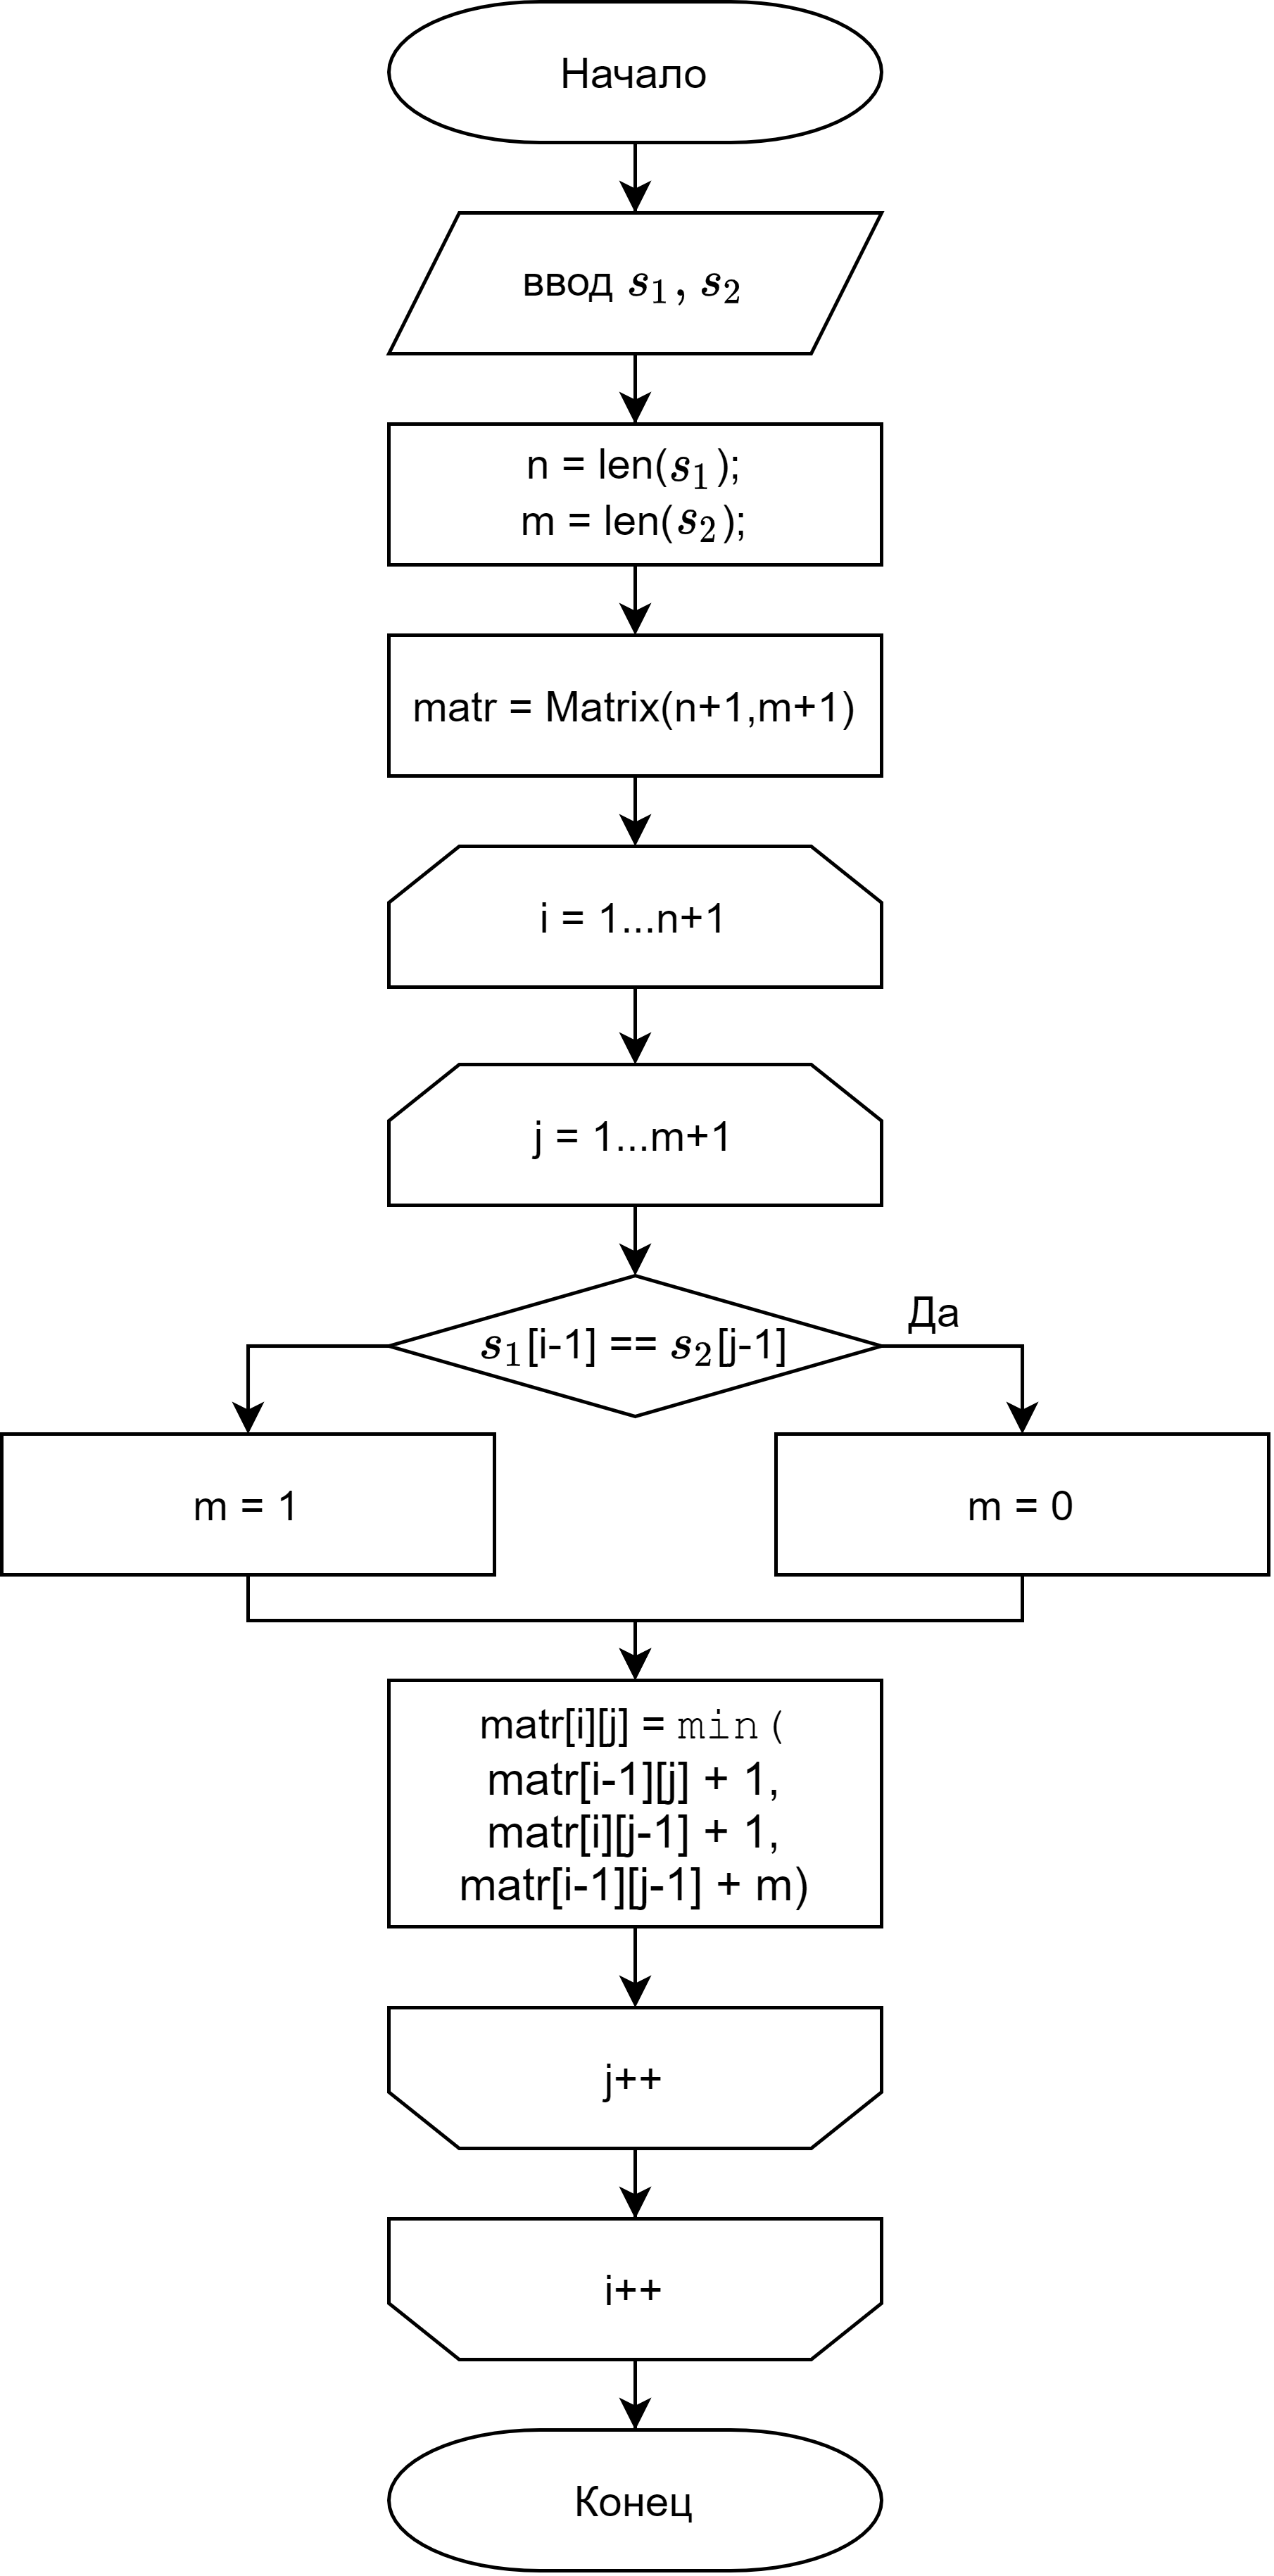
\includegraphics[scale=0.18]{LevMatr}
        \caption{Схема нерекурсивного поиска с заполнением матрицы}
        \label{schema:matr:Levenstein}
    \end{figure}

    \begin{figure}[h!]
        \centering
        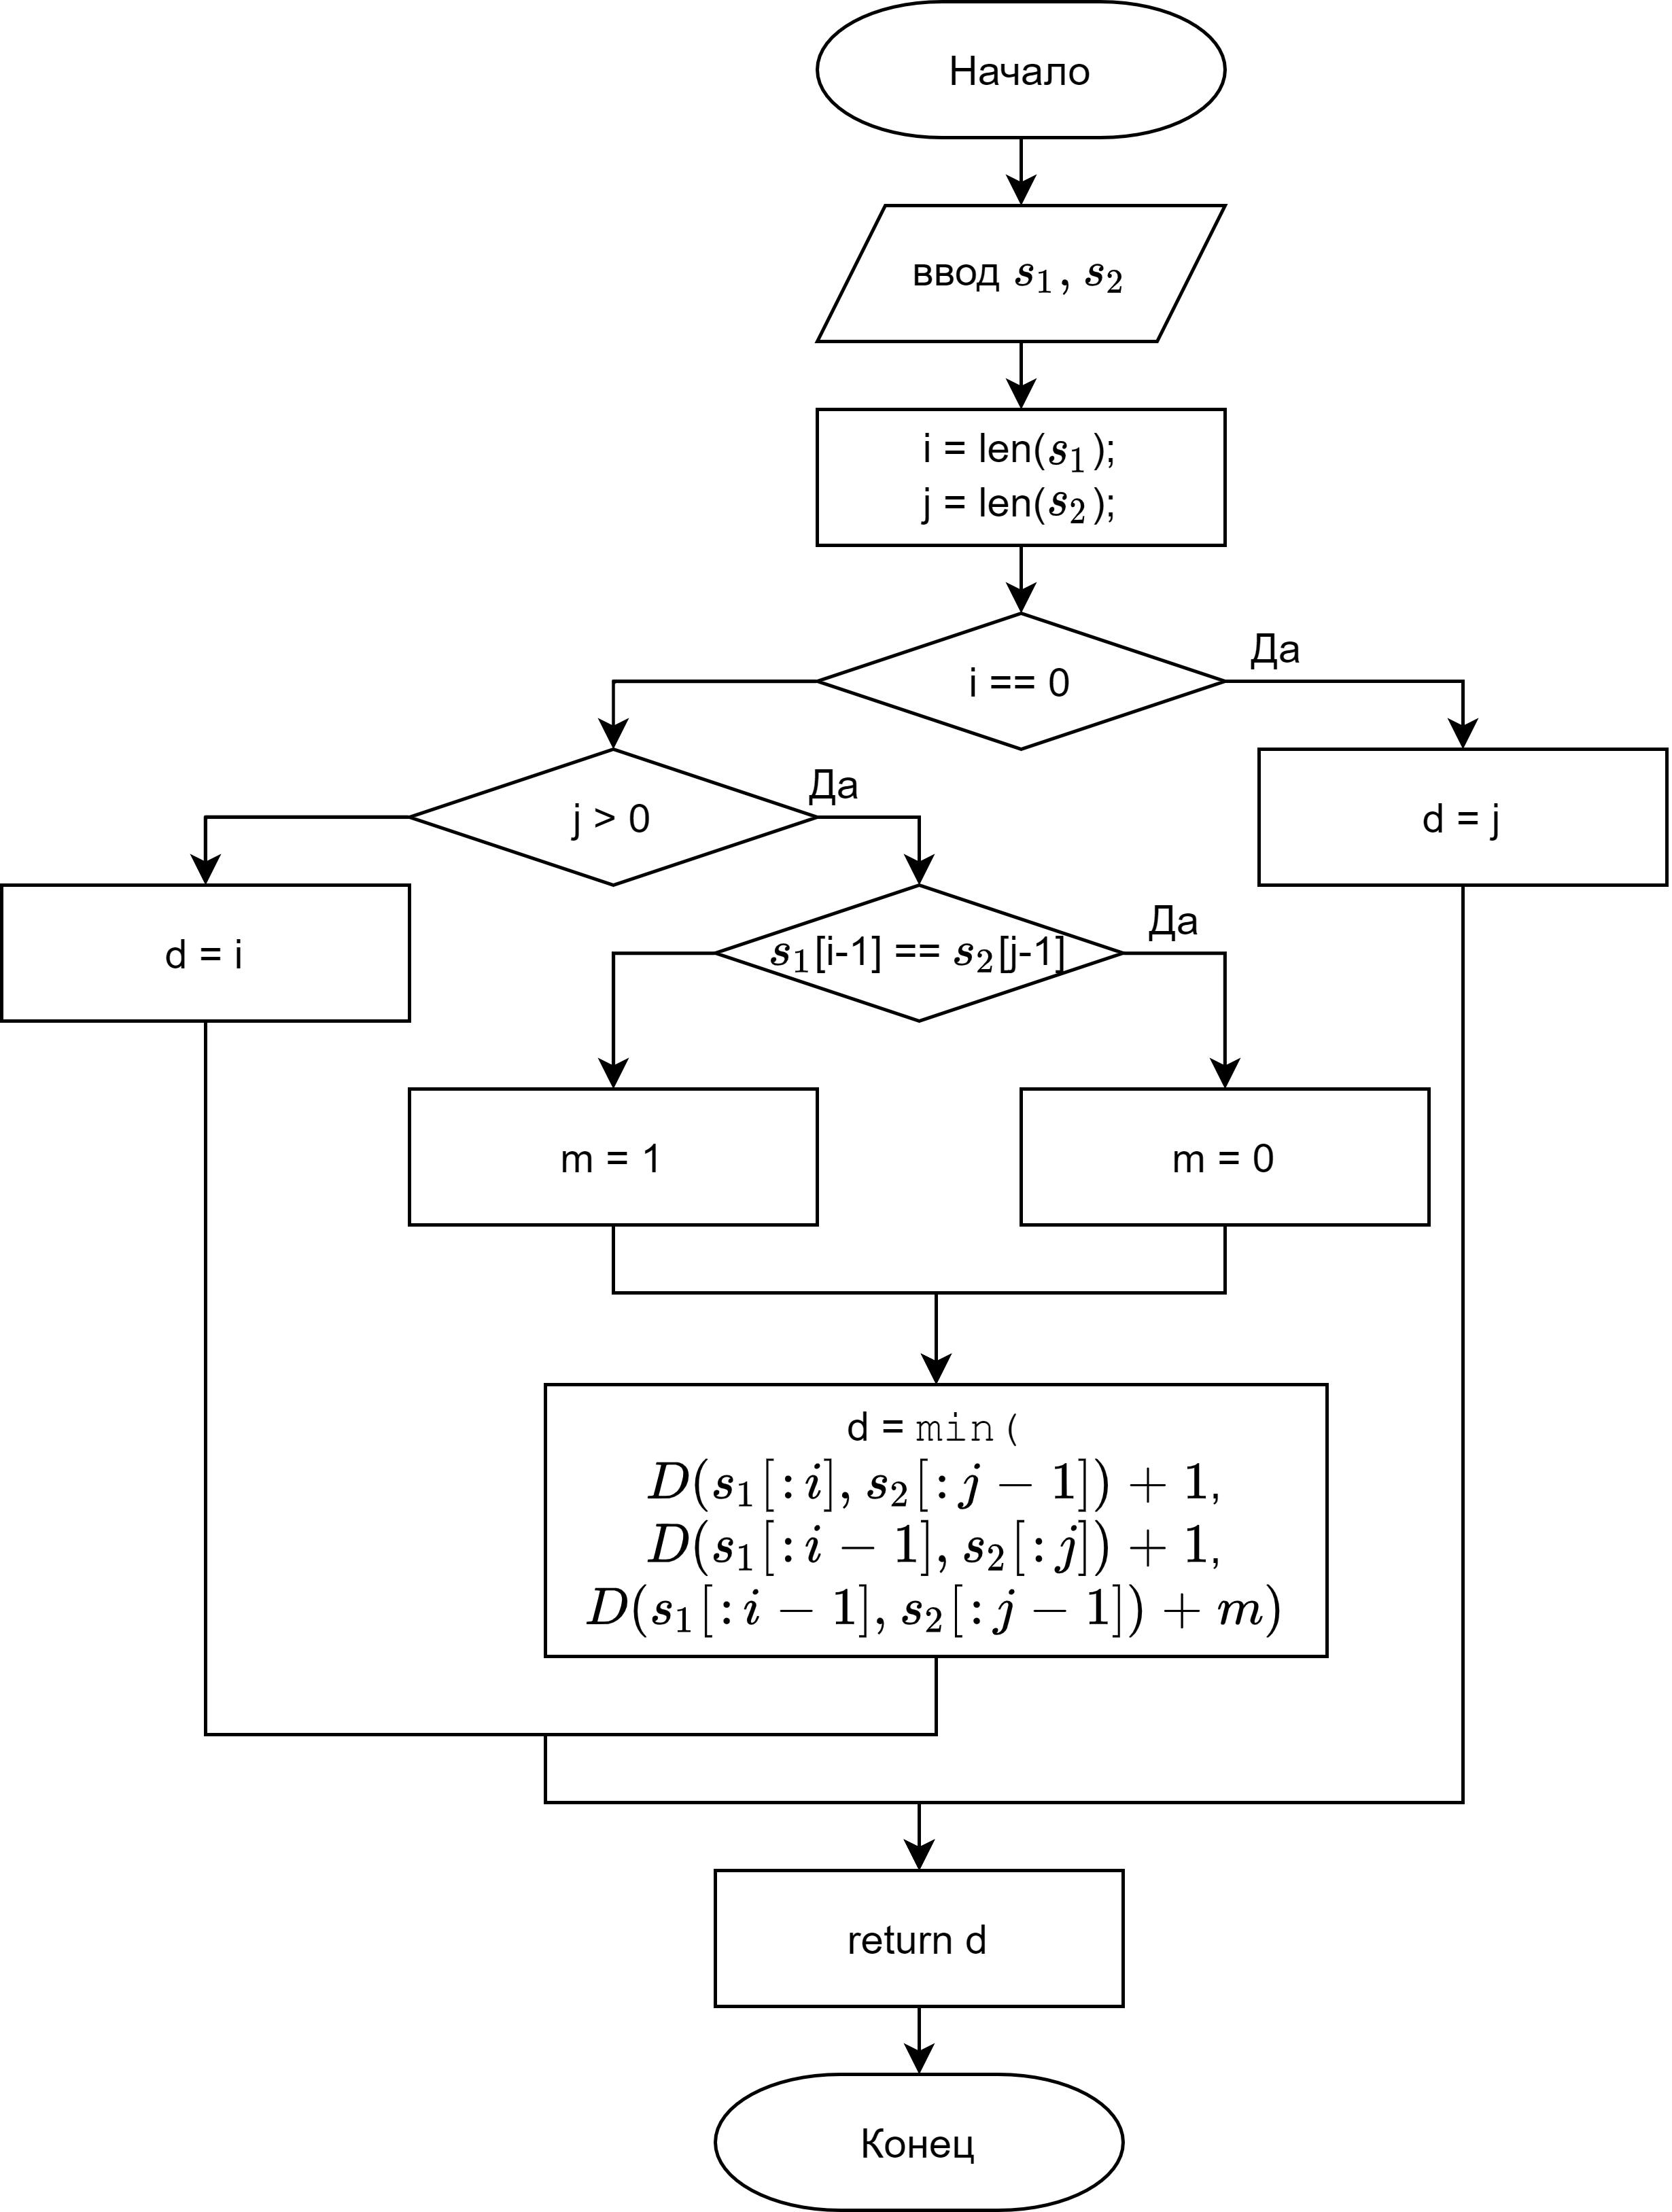
\includegraphics[scale=0.16]{LevRec}
        \caption{Схема рекурсивого поиска без заполнения матрицы}
        \label{schema:rec:Levenstein}
    \end{figure}

    \begin{figure}[h!]
        \centering
        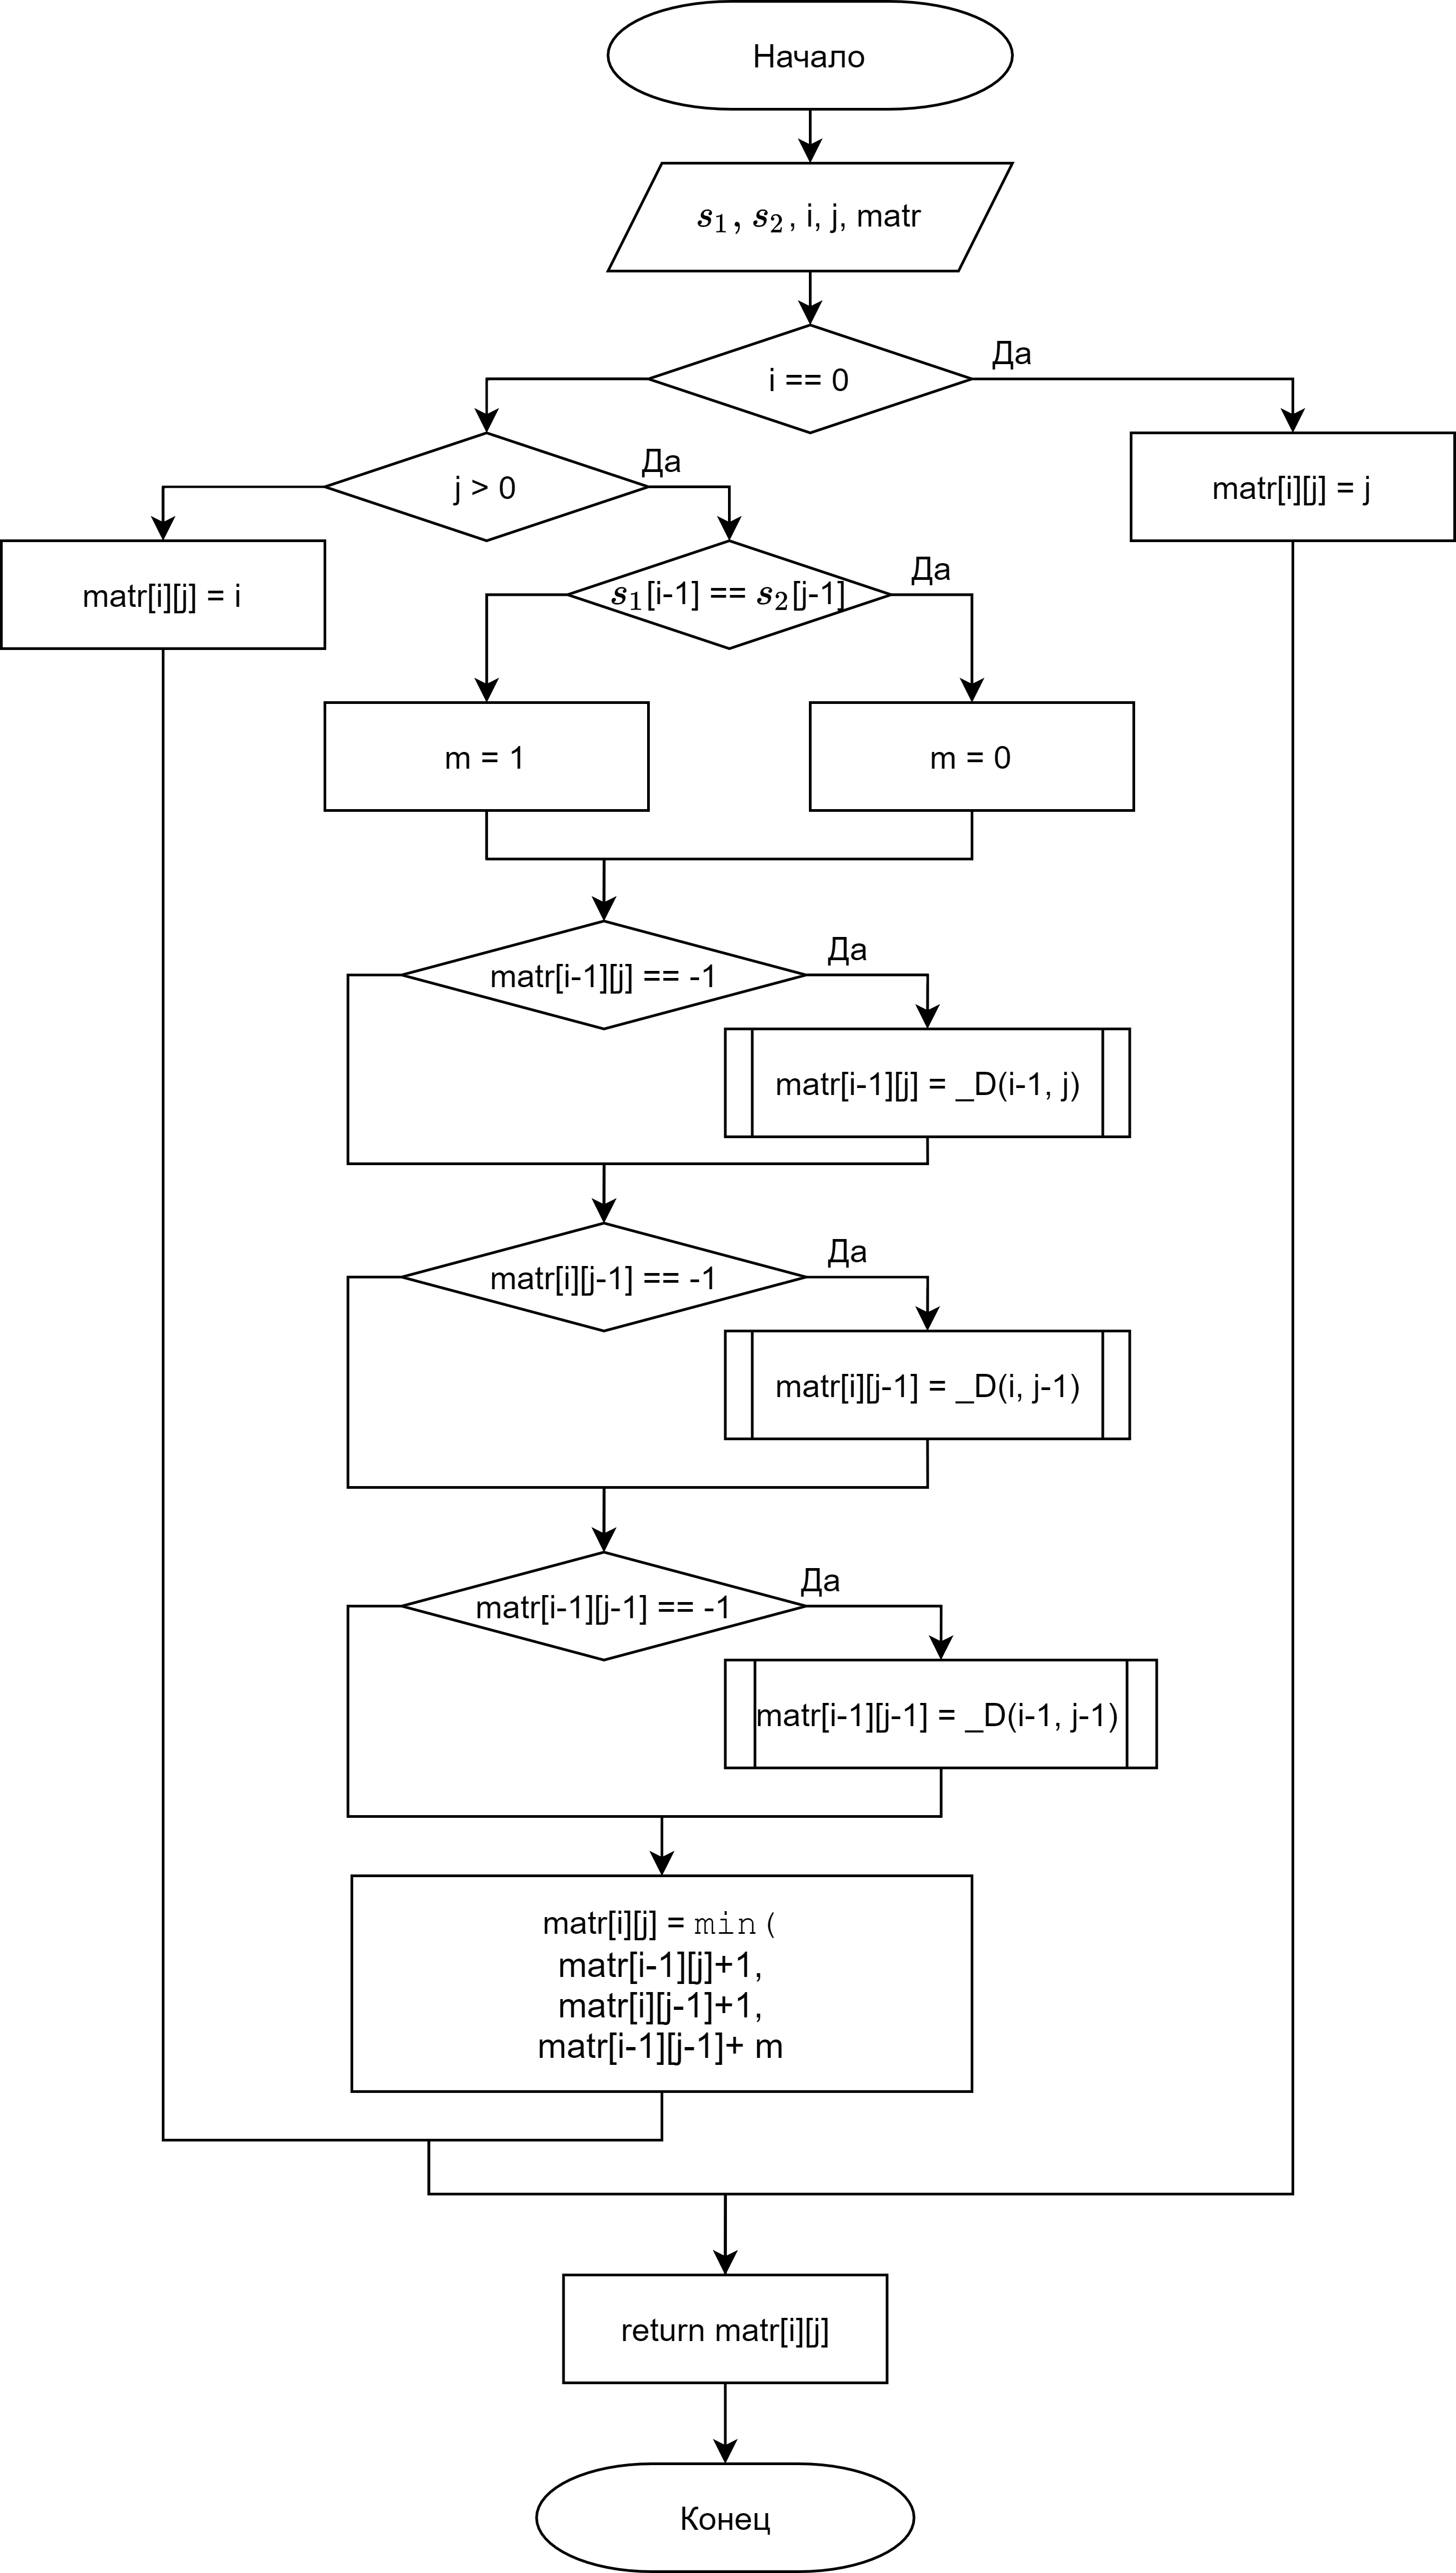
\includegraphics[scale=0.15]{LevRecMatr}
        \caption{Схема рекурсивого поиска с заполнением матрицы}
        \label{schema:rec-matr:Levenstein}
    \end{figure}

    \begin{figure}[h!]
        \centering
        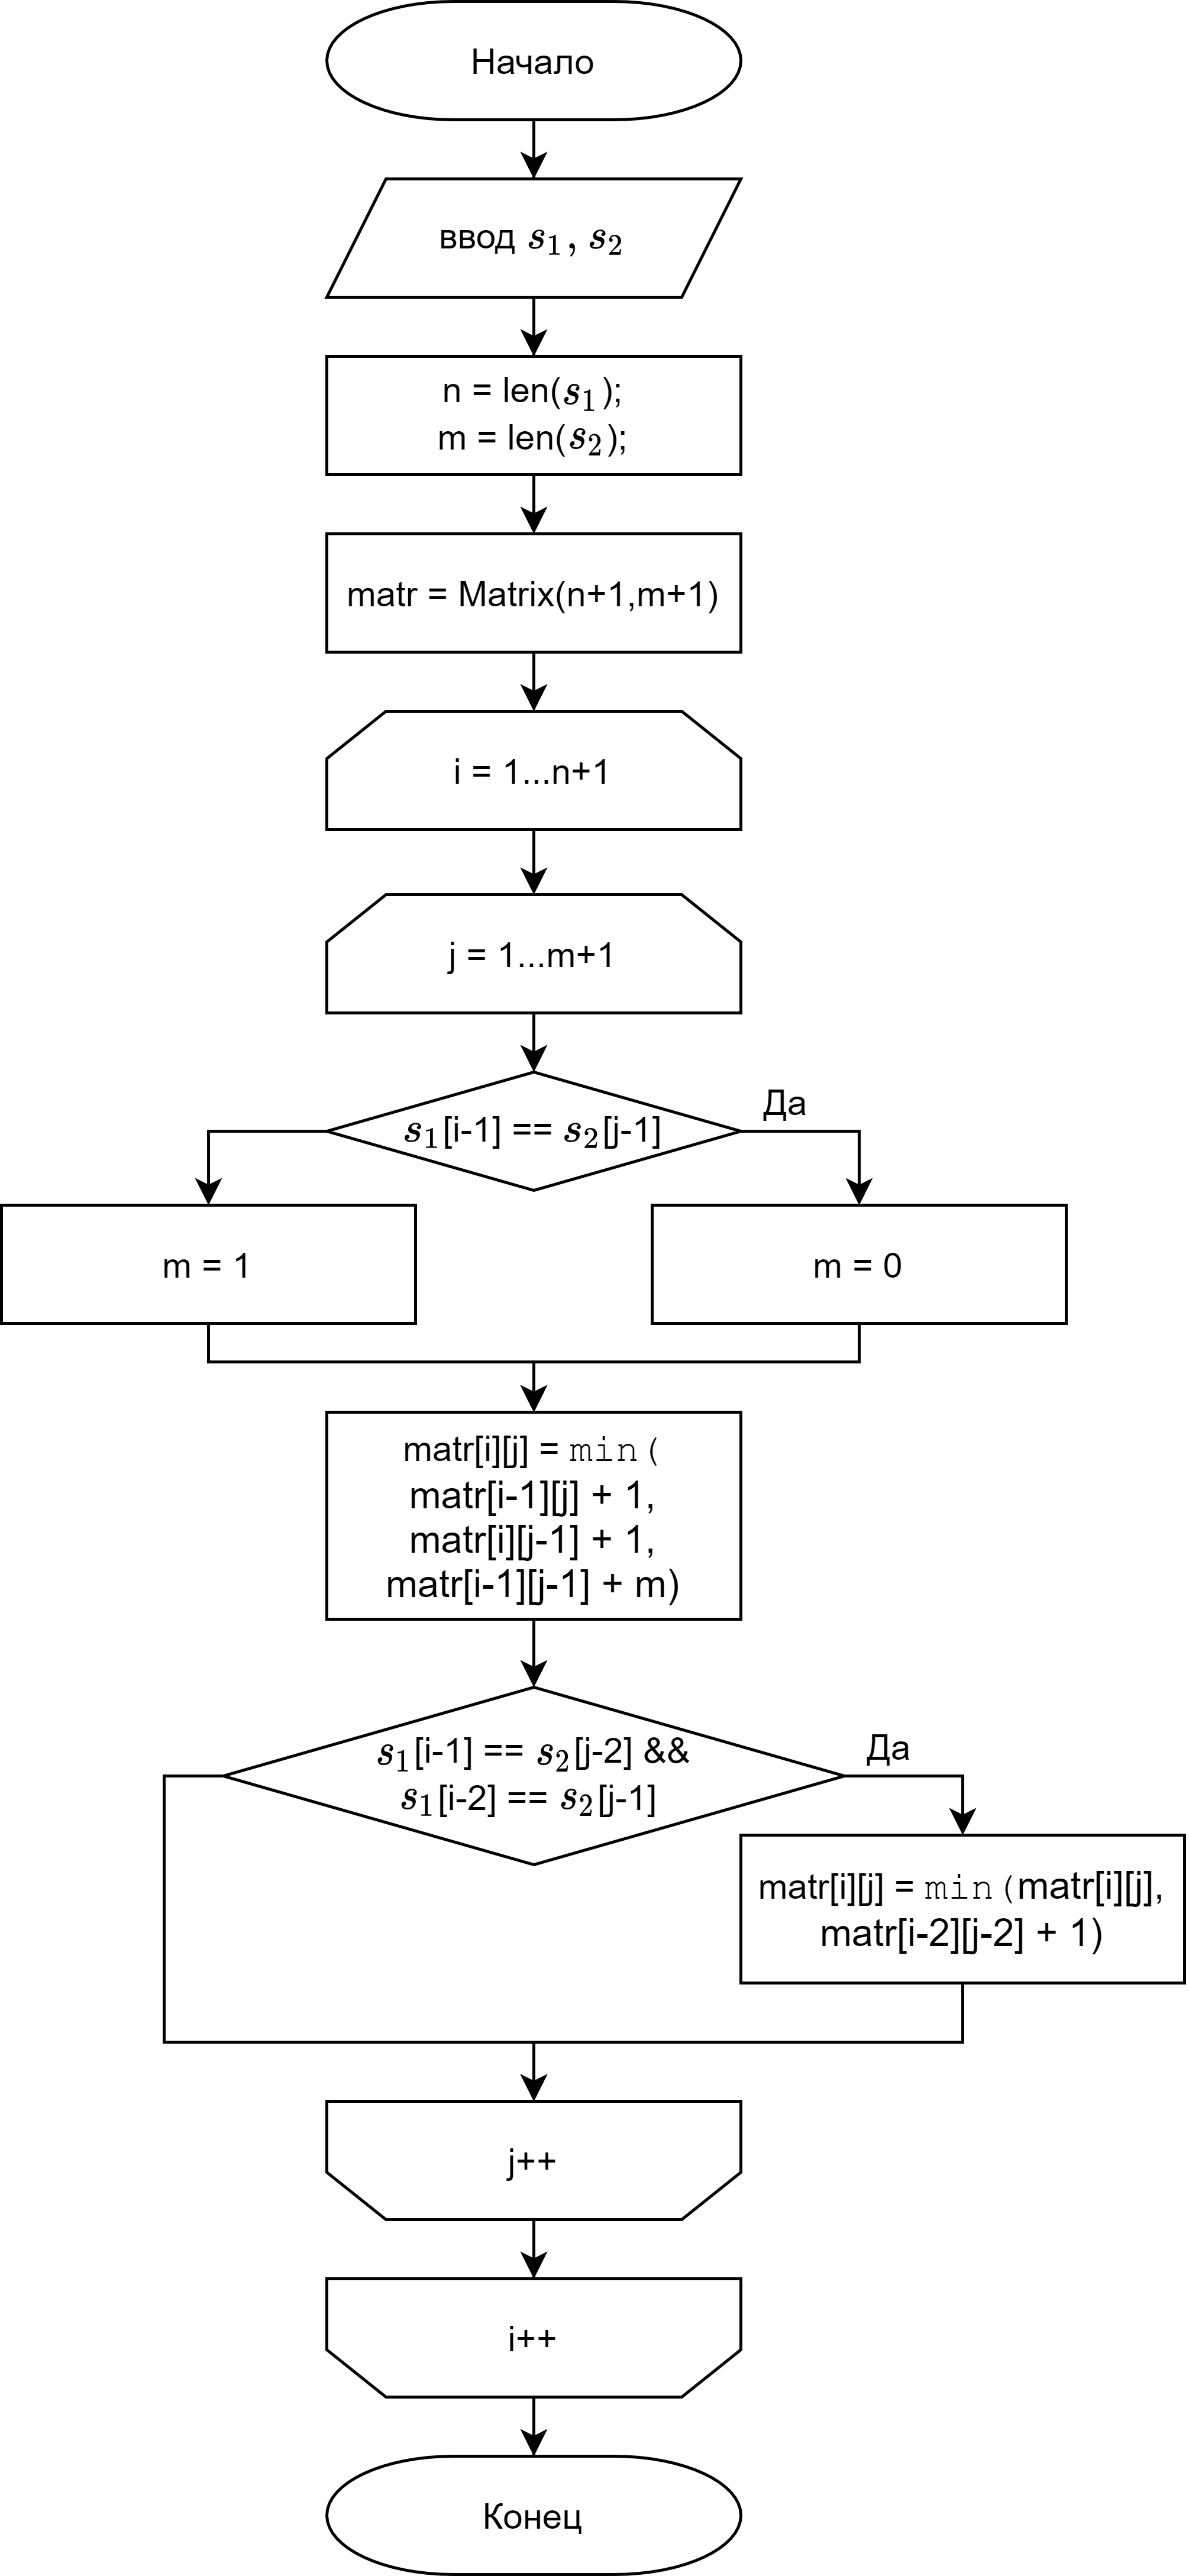
\includegraphics[scale=0.145]{DamLevMatr}
        \caption{Схема нерекурсивного поиска растояния Дамерау-Левенштейна}
        \label{schema:matr:Dameray-Levenstein}
    \end{figure}

\chapter{Технологическая часть}
В данном разделе будут выбраны средства реплизации ПО, представлен листинг кода
и проведён теоритический анализ максимальной затрачиваемой памяти.
\section{Средства реализации}
Для реализации программ я выбрал язык программирования C++, так как имею большой опыт работы с ним.
Для замера процессорного времени была использована ассемблерная вставка\cite{link_time}.

    \section{Листинг программы}
        Ниже представлены листинги кода поиска растояния Левенштейна: \begin{enumerate}
            \item нерекурсивного с заполнением матрицы (листинг \ref{levmatr});
            \item рекурсивного без заполнения матрицы (листинг \ref{levrec});
            \item рекурсивного с заполнением матрицы (листинг \ref{levrecmatr}).
        \end{enumerate}
        
        И код функции поиска растояния Дамерау-Левенштейна (листинг \ref{damerau}).

\begin{lstlisting}[label=levmatr,caption=Функция нахождения расстояния Левенштейна матрично, escapechar=@]
int LevDist(string str1, string str2)
{
    vector<vector<int>> *DistMatr = CreateMatrForLevDist(str1.size() + 1, str2.size() + 1);

    for (int i = 1; i < (@*@DistMatr).size(); i++)
    {
        for (int j = 1; j < (*DistMatr)[i].size(); j++)
        {
            (*DistMatr)[i][j] = min((*DistMatr)[i - 1][j] + 1,
                                min((*DistMatr)[i][j - 1] + 1,
                                    (*DistMatr)[i - 1][j - 1]+ (str1[i - 1] == str2[j - 1] ? 0 : 1)));
        }
    }

    int dist = (*DistMatr)[str1.size()][str2.size()];

    FreeLevDistMatr(DistMatr);

    return dist;
}
\end{lstlisting}

\newpage
\begin{lstlisting}[label=levrec,caption=Функция нахождения расстояния Левенштейна рекурсивно без матрицы]
int RLevDist(string str1, string str2)
{
    if (str1 == "" or str2 == "")
    {
        return abs((int)(str1.size() - str2.size()));
    }

    return min(RLevDist(str1.substr(0, str1.size() - 1), str2) + 1,
           min(RLevDist(str1, str2.substr(0, str2.size() - 1)) + 1,
               RLevDist(str1.substr(0, str1.size() - 1), str2.substr(0, str2.size() - 1))
               + (str1[str1.size() - 1] == str2[str2.size() - 1] ? 0 : 1)));
}
\end{lstlisting}


\begin{lstlisting}[label=levrecmatr,caption=Функция нахождения расстояния Левенштейна рекурсивно с матрицей, escapechar=@]
int RMatrLevDist_RECURSION2(string str1, string str2, vector<vector<int>> *DistMatr)
{
    if (str1.size() == 0)
    {
        (@*@DistMatr)[str1.size()][str2.size()] = str2.size();
    }
    else if (str2.size() == 0)
    {
        (*DistMatr)[str1.size()][str2.size()] = str1.size();
    }
    else
    {
        if ((*DistMatr)[str1.size()][str2.size() - 1] == -1)
        {
            (*DistMatr)[str1.size()][str2.size() - 1] = RMatrLevDist_RECURSION2(str1, str2.substr(0, str2.size() - 1), DistMatr);
        }

        if ((*DistMatr)[str1.size() - 1][str2.size()] == -1)
        {
            (*DistMatr)[str1.size() - 1][str2.size()] = RMatrLevDist_RECURSION2(str1.substr(0, str1.size() - 1), str2, DistMatr);
        }

        if ((*DistMatr)[str1.size() - 1][str2.size() - 1] == -1)
        {
            (*DistMatr)[str1.size() - 1][str2.size() - 1] = RMatrLevDist_RECURSION2(str1.substr(0, str1.size() - 1),
															str2.substr(0, str2.size() - 1), DistMatr);
        }

        int value = (str1[str1.size() - 1] == str2[str2.size() - 1] ? 0 : 1);
        (*DistMatr)[str1.size()][str2.size()] = min((*DistMatr)[str1.size() - 1][str2.size()] + 1, min((*DistMatr)[str1.size()][str2.size() - 1] + 1, (*DistMatr[str1.size() - 1][str2.size() - 1] + value));

    }
    return (*DistMatr)[str1.size()][str2.size()];
}
int RMatrLevDist(string str1, string str2)
{
    vector<vector<int>> *DistMatr = CreateMatrForLevDist2(str1.size() + 1, str2.size() + 1);

    int dist = RMatrLevDist_RECURSION2(str1, str2, DistMatr);

    FreeLevDistMatr(DistMatr);

    return dist;
}

\end{lstlisting}


\begin{lstlisting}[label=damerau,caption=Функция нахождения расстояния Дамерау-Левенштейна матрично, escapechar=@]
int Dam_LevDist(string str1, string str2)
{
    vector<vector<int>> *DistMatr = CreateMatrForLevDist(str1.size() + 1, str2.size() + 1);

    for (int i = 1; i < (@*@DistMatr).size(); i++)
    {
        for (int j = 1; j < (*DistMatr)[i].size(); j++)
        {
            (*DistMatr)[i][j] = min((*DistMatr)[i - 1][j] + 1,
                                min((*DistMatr)[i][j - 1] + 1,
                                    (*DistMatr)[i - 1][j - 1] + (str1[i - 1] == str2[j - 1] ? 0 : 1)));

            if ((i > 1 and j > 1) and str1[i - 1] == str2[j - 2] and str1[i - 2] == str2[j - 1])
            {
                (*DistMatr)[i][j] = min((*DistMatr)[i][j], (*DistMatr)[i - 2][j - 2] + 1);
            }
        }
    }

    int dist = (*DistMatr)[str1.size()][str2.size()];

    FreeLevDistMatr(DistMatr);

    return dist;
}
\end{lstlisting}

\section{Тестирование}
В таблице \ref{table:testing} отображён возможный набор тестов для тестирования методом чёрного ящика.
В столбцах "Ожидаемый результат" и "Полученный результат"  4 числа соответсвуют рекурсивному алгоритму без матрицы нахождения расстояния Левенштейна, рекурсивному алгоритму с матрицей нахождения расстояния Левенштейна, матричному алгоритму нахождению расстоянию Левенштейна, матричному алгоритму нахождения расстояние Дамерау-Левенштейна.

\begin{table}[]
            \caption{Таблица тестовых данных}
            \centering
            \begin{tabular}{|c|c|c|c|c|}
            \hline
            № & строка 1 & строка 2 & \begin{tabular}[c]{@{}c@{}}Ожидаемый результат \\\end{tabular} & \begin{tabular}[c]{@{}c@{}}Фактический результат\\ \end{tabular} \\ \hline
 	1 & kot & skat & 2 2 2 2 & 2 2 2 2\\
 	\hline
	2 & zxc & cxz & 2 2 2 2 &  2 2 2 2\\
	\hline
	3 & sok & kokos & 3 3 3 3 & 3 3 3 3\\
	\hline
	4 & qwerty & asdfgh & 6 6 6 6 & 6 6 6 6\\
	\hline
	5 & qwerty & qewryt & 4 4 4 2 & 4 4 4 2\\
	\hline
            \end{tabular}
            \label{table:testing}
        \end{table}


    \section{Сравнительный анализ потребляемой памяти}  
        С точки зрения использования памяти алгоритмы Левенштейна и
        Дамерау-Левенштейна не отличаются, следовательно, достаточно
        рассмотреть лишь разницу рекурсивной и матричной реализаций
        данных методов.
        
        Использование памяти на строках $s_1$, $s_2$ длиной n и m соответственно
        при использовании матрицы теоритически определяется формулой (\ref{formula:memory:matr}):
        \begin{equation}
            V = (n + 1)(m + 1)sizeof(int) + 4sizeof(size\_t) + 2sizeof(char*) + sizeof(char)(n + m)
            \label{formula:memory:matr}
        \end{equation}
        

        Максимальный расход памяти памяти на строках $s_1$, $s_2$ длиной n и m соответственно
        при использовании рекурсии определяется максимальной глибиной стека вызовов,
        которая теоритически определяется формулой (\ref{formula:memory:rec}):
        \begin{equation}
            V = sizeof(char)(n + m)  + (n + m)(2sizeof(char*) + 3sizeof(size\_t))
            \label{formula:memory:rec}
        \end{equation}




\chapter{Исследовательская часть}
    В данном разделе будут проведены эксперименты для проведения 
    сравнительного анализа алгоритмов по затрачиваемому процессорному 
    времени\cite{link2} и максимальной используемой памяти.

\section{Сравнительный анализ на основе замеров времени работы алгоритмов}

Был проведен замер времени работы каждой реализации на строках равной длинны, с их случайным заполнением.
В таблице \ref{table:time} приняты следующие обозначения:\begin{enumerate}
            \item LevRecursion -- расстояние Левенштейна (рекурсивно, без матрицы) ;
            \item LevMatrix -- расстояние Левенштейна (матрично, без рекурсии) ;
            \item LevRecursionMatrix -- расстояние Левенштейна (матрично, с рекурсией);
	    \item DamLevMatrix -- расстояние Дамерау-Левенштейна (матрично).
        \end{enumerate}

Графики по таблице изображены на рисунках \ref{graph:graph1}.

\begin{table} [h!]
\caption{Время работы реализации алгоритмов  (в наносекундах)}
	\centering
	\begin{tabular}{|c c c c c|} 
 	\hline
	len & LevMatrix & LevRecursion & LevRecursionMatrix & DamLevMatrix \\ [0.8ex] 
 	\hline\hline
 	1 & 4982 & 3024 & 6445 & 5064\\
 	\hline
 	2 & 4993 & 14832 & 10188 & 5082\\
 	\hline
	3 & 5681 & 62872 & 14739 & 5725\\
	\hline
	4 & 6325 & 302576 & 20268 & 6382\\
	\hline
	5 & 7819 & 1504108 & 27811 & 7960\\
	\hline
	\end{tabular}
	\label{table:time}
\end{table}


\begin{figure}[h!]
\centering
\begin{tikzpicture}
\begin{axis}[
    	axis lines = left,
    	xlabel={Длина (символы)},
    	ylabel={Время (наносек.)},
	legend pos=north west,
	ymajorgrids=true,
                    height = 0.5\paperheight, 
                    width = 0.75\paperwidth
]



\addplot table [x = b, y = a] { 
	b      a
1 4982
2 4993
3 5681
4 6325
5 7819
};

\addplot table [x = b, y = a] {
	b      a
1 3024
2 14832
3 62872
4 302576
};

\addplot table [x = b, y = a] { 
	b      a
1 6445
2 10188
3 14739
4 20268
5 27811
};

\addplot table [x = b, y = a] {
	b      a
1 5064
2 5082
3 5725
4 6382
5 7960
};


\legend{
                    р. Левенштейна не рекурсивный с заполнением матрицы,
                    р. Левенштейна рекурсивный без заполнения матрицы,
                    р. Левенштейна рекурсивный с заполнением матрицы,
                    р. Дамерау-Левенштейна не рекурсивный
                };

\end{axis}
\end{tikzpicture}
\caption{График зависимости времени работы алгоритмов от длин строк} 
\label{graph:graph1}
\end{figure}


\par
Наиболее эффективными по времени при маленькой длине слова являются рекурсивные реализации алгоритмов, но как только увеличивается длина слова, их эффективность резко снижается, что обусловлено большим количеством повторных рассчетов. Время работы алгоритма, использующего матрицу, намного меньше благодаря тому, что в нем требуется только (m + 1)*(n + 1) операций заполнения ячейки матрицы. Также установлено, что алгоритм Дамерау-Левенштейна работает немного дольше алгоритма Левенштейна, т.к. в нем добавлены дополнительные проверки, однако алгоритмы сравнимы по временной эффективности.


\chapter*{Заключение}
\addcontentsline{toc}{chapter}{Заключение}
Был изучен метод динамического программирования на материале алгоритмов Левенштейна и Дамерау-Левенштейна.
Также изучены алгоритмы Левенштейна и Дамерау-Левенштейна нахождения расстояния между строками, получены практические навыки раелизации указанных алгоритмов в матричной  и рекурсивных версиях. 

Экспериментально было подтверждено различие во временной эффективности рекурсивной и нерекурсивной реализаций выбранного алгоритма определения расстояния между строками при помощи разработаного программного обеспечения на материале замеров процессорного времени выполнения реализации на варьирующихся длинах строк. 

В результате исследований я пришел к выводу, что матричная реализация данных алгоритмов заметно выигрывает по времени при росте длины строк, следовательно более применима в реальных проектах.
 
%далее сам список используевой литературы
\begin{thebibliography}{}
    \bibitem{link_time}  Ассемблерные вставки в AVR-GCC. // [Электронный ресурс]. Режим доступа: http://we.easyelectronics.ru/AVR/assemblernye-vstavki-v-avr-gcc.html, (дата обращения: 03.10.2020).
    \bibitem{link2}  C/C++: как измерять процессорное время. // [Электронный ресурс]. Режим доступа: https://habr.com/ru/post/282301/, (дата обращения: 03.10.2020).
\end{thebibliography}

\end{document}